% Results and Discussion: Insertable Figures and Tables
% Requires: \usepackage{graphicx}, \usepackage{booktabs}, \usepackage{siunitx}
% Optional: \usepackage{caption}

% ---------- Figure: Pareto Front (ε-Constraint) ----------
% If you generated a dedicated Pareto front image, set the path below.
\begin{figure}[h]
  \centering
  % 
\includegraphics[width=0.9\linewidth]{Output Data/pareto_front_fuel_optimization.png}
  % Fallback: use comparison overlay if single-front image not available
  
\includegraphics[width=0.9\linewidth]{Output Data/pareto_front_comparison.png}
  \caption{Pareto Front(s): Cost vs Strategic Supplier Score.}
  \label{fig:pareto_front}
\end{figure}

% ---------- Table: Representative ε-Constraint Solutions ----------
% Extracted from latest e-constraint front (Output Data/econstraint_front_20250929T161217Z.csv)
\begin{table}[h]
  \centering
  \caption{Representative Pareto Solutions (ε-Constraint). Costs in Rands; deltas vs Min Cost.}
  \label{tab:rep_solutions}
  \sisetup{round-mode=places,round-precision=2,group-separator=\,}
  \begin{tabular}{l S S S[round-precision=4] S S[round-precision=2]}
    \toprule
    {Point} & {Cost (R)} & {Strategic Score} & {$\Delta$Cost (R)} & {$\Delta$Cost (\%)} & {$\Delta$Score (\%)} \\
    \midrule
    Min Cost   & 1290475652.50 & 4047 & 0 & 0.0000 & 0.00 \\
    Knee       & 1290481476.39 & 4249 & 5823.89 & 0.0005 & 4.99 \\
    Max Score  & 1290970044.28 & 4550 & 494391.78 & 0.0383 & 12.43 \\
    \bottomrule
  \end{tabular}
\end{table}

% Notes:
% - Knee identified by highest marginal gain in score per unit cost among adjacent points.

% ---------- Table: Pareto Indicators and Dominance Coverage ----------
% Extracted from Output Data/comparison_summary_20250929T161217Z.json
\begin{table}[h]
  \centering
  \caption{Pareto Indicators and Pairwise Coverage (Latest Run).}
  \label{tab:pareto_indicators}
  \sisetup{round-mode=places,round-precision=6,group-separator=\,}
  \begin{tabular}{l S[round-precision=0] S[round-precision=3] S[round-precision=6] S[round-precision=6]}
    \toprule
    {Method} & {Points} & {Hypervolume} & {IGD} & {Spacing} \\
    \midrule
    $\epsilon$-Constraint & 27 & 301,499,191.444063 & 0.014045 & 0.084929 \\
    NSGA-II                & 78 & 298,284,566.026129 & 0.004201 & 0.034896 \\
    \bottomrule
  \end{tabular}
\end{table}

% Pairwise dominance coverage (A dominates B):
% coverage_a_dom_b = 0.384615, coverage_b_dom_a = 0.037037
% Include as text near the table if desired.

% ---------- Figure: Allocation Map (Static Snapshot) ----------
% Export a PNG snapshot of the interactive map to the path below before compiling.
\begin{figure}[h]
  \centering
  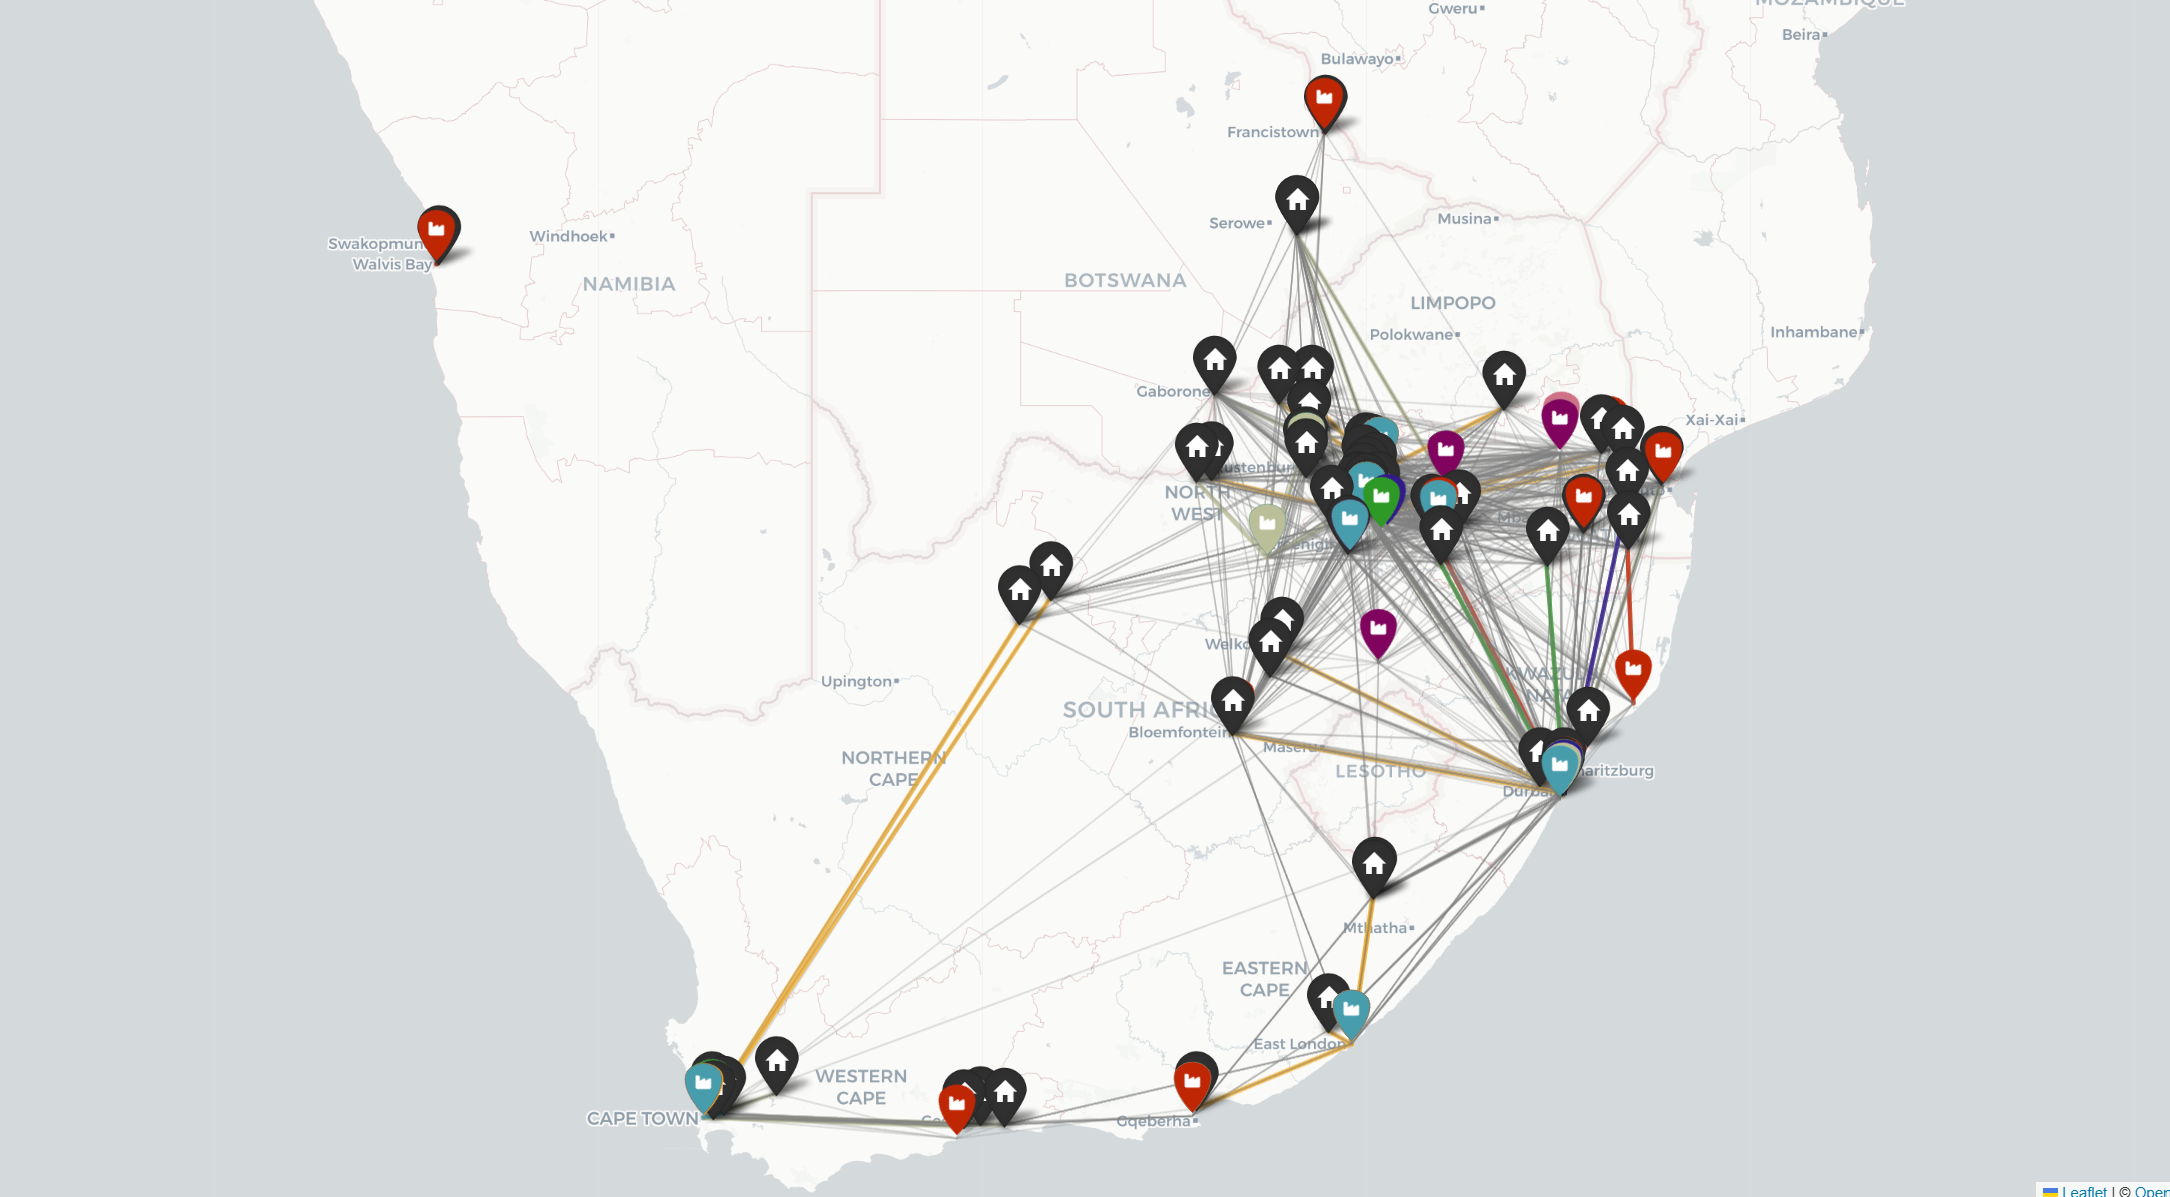
\includegraphics[width=0.95\linewidth]{final_version/chapters_copy/optimization_allocation_map.png}
  \caption{Optimized Allocation Map (Cost-Only Baseline). Node color by supplier, line thickness by volume.}
  \label{fig:allocation_map}
\end{figure}

% ---------- Table (Placeholder): Supplier Utilization Summary ----------
% Fill from cost-only baseline run aggregation in fuel_optimizer_docplex.py results.
\begin{table}[h]
  \centering
  \caption{Supplier Utilization Summary (Cost-Only Baseline).}
  \label{tab:supplier_utilisation}
  \begin{tabular}{l r r r r}
    \toprule
    Supplier & Allocations & Total Volume (L) & Total Cost (R) & Avg Cost/L (R) \\
    \midrule
    % TODO: Fill from baseline run results
    \bottomrule
  \end{tabular}
\end{table}

% ---------- Table (Placeholder): Capacity Constraints Summary ----------
% Fill from binding/near-capacity outputs in fuel_optimizer_docplex.py results.
\begin{table}[h]
  \centering
  \caption{Supplier Depot Capacity Constraints Summary.}
  \label{tab:capacity_summary}
  \begin{tabular}{l r r r}
    \toprule
    Supplier Depot (ID) & Used Volume (L) & Capacity Limit (L) & Utilisation (\%) \\
    \midrule
    % TODO: Fill from baseline run results
    \bottomrule
  \end{tabular}
\end{table}
